% LAB 4: Lists and Strings
%
% CSE/IT 107: Introduction to Programming
% New Mexico Tech
%
% Prepared by Russell White and Christopher Koch
% Fall 2014
\documentclass[11pt]{cselabheader}

%%%%%%%%%%%%%%%%%% SET TITLES %%%%%%%%%%%%%%%%%%%%%%%%%
\fancyhead[R]{Lab 4: Lists and Strings}
\title{Lab 4: Lists and Strings}

\begin{document}

\maketitle

\hrule

\begin{quotation}
``Programming is learned by writing programs.''
\end{quotation}
\begin{flushright}
--- Brian Kernighan
\end{flushright}

\begin{quotation}
``The purpose of computing is insight, not numbers.''
\end{quotation}
\begin{flushright}
--- Richard Hamming, 1962
\end{flushright}

\begin{quotation}
  ``From our own history we learn what man is capable of. For that reason we
  must not imagine that we are quite different and have become better.''
\end{quotation}
\begin{flushright}
	--- Richard von Weizs\"{a}cker
%\\\textit{Speech to commemorate end of WW II, May 8 1985}
% English: http://www.hariguchi.org/yoichi/weizsaecker.html
% Famous speech by RvW, President of Fed Rep of Germ, for the 
% commemoration of the 40th anniversary of the end of WWII in
% Germany on May 8, 1985
% German: http://www.hdg.de/lemo/html/dokumente/NeueHerausforderungen_redeVollstaendigRichardVonWeizsaecker8Mai1985/index.html
\end{flushright}
\hrule

\section{Introduction}
In the first two labs, we showed you how to generally use Python and how to
have your programs make decisions based on what the user entered. With this
lab, we will be starting to show you how to do some useful things in Python:
how to make lists and manipulate them -- sort them, reverse them, combine them.
We will also show you how to deal with strings. You have
seen strings before, but we will be showing you how to manipulate them.

\pagebreak
\section{Lists}
%in/not in, slicing, pop, append, len, sum
One of the most important data types in Python is the list. A list is an ordered
collection of other values. For example, we might create a list of numbers
representing data points on a graph or create a list of strings representing
students in a class. Creating a list is simple. We simply place comma-separated
values inside square brackets.

\begin{pyconcode}
>>> values = [1, 2, 3, 4, 5]
>>> print(values)
[1, 2, 3, 4, 5]
\end{pyconcode}

\subsection{Indices}
Once we put a value in a list, we can treat the list as a single entity or
access individual values. In order to access an individual element, we need to
use the index of the value we want to access. The index is the position of the
element in the list if we start numbering the elements from 0. When we are
accessing list elements by index we can use them in any way we might use a
normal variable.

\begin{pyconcode}
>>> values = [23, 7, 18, 0.23, 91]
>>> print(values[0])
23
>>> print(values[2])
18
>>> print(values[3])
0.23
>>> values[3] = 7.5
>>> print(values[3])
7.5
>>> print(values)
[23, 7, 18, 7.5, 91]
>>> values[0] = values[0] + values[1]
>>> print(values)
[30, 7, 18, 7.5, 91]
\end{pyconcode}

If we wish, we can use negative array indices to reference elements starting at
the end of the list. For example, -1 is the last element, -2 is the second to
last element, and so on.

\begin{pyconcode}
>>> values = [32, 1, 54, -3, 6]
>>> print(values[-1])
6
>>> print(values[-2])
-3
\end{pyconcode}

\subsection{Values in Lists}
We can use an existing variable when creating a list. If we change the value of
the variable, the value in the list will stay the same.

\begin{pyconcode}
>>> x = 35
>>> k = 19
>>> y = 5
>>> values = [x, k, y]
>>> print(values)
[35, 19, 5]
>>> x = 1
>>> print(values)
[35, 19, 5]
\end{pyconcode}

All values in a list do not need to be the same type. If we want, we can create
a list with both numbers and strings, although this is usually a poor idea.

\begin{pyconcode}
>>> values = [2, 'hello', 5.3]
>>> print(values)
[2, 'hello', 5.3]
\end{pyconcode}

If you want, you can even put a list inside a list!

\begin{pyconcode}
>>> values = [1, 5, 2]
>>> more_values = [7, 'test', values]
>>> print(more_values)
[7, 'test', [1, 5, 2]]
>>> print(more_values[2])
[1, 5, 2]
\end{pyconcode}

Note that, unlike with other variables, changing an element of a list inside
another list will change both values.

\begin{pyconcode}
>>> values = [1, 5, 2]
>>> more_values = [7, 'test', values]
>>> print(more_values)
[7, 'test', [1, 5, 2]]
>>> values[2] = 7
>>> print(more_values)
[7, 'test', [1, 5, 7]]
>>> values = [1, 2]
>>> print(more_values)
[7, 'test', [1, 5, 7]]
\end{pyconcode}

You generally will not have to worry about this, though the reason is because we
are modifying the existing value rather than create a new list. When we reassign
\pythoninline{values}, it no longer changes the values inside inside
\pythoninline{more_values}. This is because we are creating a new list for
\pythoninline{values} rather than modifying the existing list.

\subsection{Testing List Contents}
A common operation is to test if a list contains a given value. We can do this
using the \pythoninline{in} keyword. We can also test if a list does not contain a
value using \pythoninline{not in}.

\begin{pyconcode}
>>> values = [1, 'test', 30, 20]
>>> print(1 in values)
True
>>> print('test' in values)
True
>>> print(2 in values)
False
>>> print(2 not in values)
True
\end{pyconcode}

This could be used to simplify the example from Lab 2 involving checking user
input against multiple valid passwords.

\begin{python3code}
passwords = ['hunter2', 'hunter3', 'hunter4']

user_in = input('Please enter your password: ')

if user_in in passwords:
    print('Correct password. Welcome!')
else:
    print('Incorrect password.')
\end{python3code}

\subsection{Slicing}
Often we will want to make a new list out of part of a larger list. We do this
using slicing. To do this, we specify the first and last indices we want to
include in our new list, separated by a colon. The last index is used as a
bookend -- that is, values up to but not including that index are included in
the new list. If one of the values is omitted, then Python will act as if the
most extreme index on that side was enterred. Omitting both values will use the
full list.

Thus, for a list \pythoninline!L! and two positions (indices) \pythoninline!B! and
\pythoninline!E! within that list, the expression \pythoninline!L[ B : E ]! produces a
new list containing the elements in \pythoninline!L! between those two positions
not including \pythoninline!E!. Notice that \pythoninline!B! and \pythoninline!E! must be
indices -- whole numbers.

\begin{pyconcode}
>>> L = [1, 2, 3, 4, 5]
>>> print(L[1:3])
[2, 3]
>>> print(L[3])
4
\end{pyconcode}

Note that \pythoninline!L[1:3]! did \emph{not} include \pythoninline!L[3]!. 

You may omit the starting position to slice elements from the beginning of the
list up to the specified position. You may similarly omit the ending position to
specify that a slice extends to the end of the list. You can even omit both of
them to just get a copy of the whole list.

\begin{pyconcode}
>>> print(L[:3])
[1, 2, 3]
>>> print(L[1:])
[2, 3, 4, 5]
>>> print(L[:])
[1, 2, 3, 4, 5]
\end{pyconcode}

Using slicing allows us to add or delete elements from lists:

\begin{pyconcode}
>>> L = [1, 2, 3, 4, 5]
>>> L[2:4] = [93, 94, 95, 96]
>>> print(L)
[1, 2, 93, 94, 95, 96, 5]
>>> L[3:6] = []
[1, 2, 93, 5]
\end{pyconcode}

If we include an additional colon and value, we can include a step size. For
example, a step size of two will create the list from every other value in the
original list. A negative step size allows the list to be reversed.

Then, given a list \pythoninline!L! and two positions (indices) \pythoninline!B! and
\pythoninline!E! as well as a step size \pythoninline!S!, you can use the expression
\pythoninline!L[ B : E : S]! to obtain the elements of \pythoninline!L! between
\pythoninline!B! and \pythoninline!E! positions in increments of \pythoninline!S!
positions.

\begin{pyconcode}
>>> values = [1, 2, 3, 4, 5]
>>> print(values[::2])
[1, 3, 5]
>>> print(values[1:4:2])
[2, 4]
>>> print(values[4:1:-1])
[5, 4, 3]
\end{pyconcode}

\subsection{List Functions}
Many functions exist to help manipulate lists. The first of these is
\pythoninline{.append()}. This adds a new value onto the end of an existing list.

\begin{pyconcode}
>>> values = [1, 2, 3]
>>> values.append(12)
>>> values.append(123)
>>> print(values)
[1, 2, 3, 12, 123]
\end{pyconcode}

\pythoninline{.insert()} also inserts a value, but it allows you to choose where it
goes. The first argument of the function is the index you want your new value to
be located. Other values will be moved to make room.

\begin{pyconcode}
>>> values = [1, 2, 3, 4]
>>> values.insert(2, 10)
>>> print(values)
[1, 2, 10, 3, 4]
\end{pyconcode}

The \pythoninline{.pop()} function works similarly to accessing list values by
index, but also removes the element from a list. If given a value, then
\pythoninline{.pop()} will remove the value at that index. If not, it will remove
the last value in the list.

\begin{pyconcode}
>>> values = [1, 2, 3, 12, 123]
>>> print(values.pop())
123
>>> print(values.pop(0))
1
>>> print(values)
[2, 3, 12]
\end{pyconcode}


Using \pythoninline{len} returns the length of the list passed to it.

\begin{pyconcode}
>>> values = [1, 2, 3, 12, 123]
>>> print(len(values))
5
\end{pyconcode}

\pythoninline{sum} allows the easy summing of every value in a list, so long as
every value in the list is a number. If any values are not, an error will occur.

\begin{pyconcode}
>>> values = [1, 2, 3, 12, 123]
>>> print(sum(values))
141
>>> values.append('test')
>>> print(sum(values))
Traceback (most recent call last):
  File "<stdin>", line 1, in <module>
TypeError: unsupported operand type(s) for +: 'int' and 'str'
\end{pyconcode}

\begin{table}[!ht]
  \centering
  \begin{tabular}{ll}
    \toprule
    Function & What it does \\
    \midrule
    \pythoninline!lst.append(x)! & appends \pythoninline!x! to \pythoninline!lst! \\
    \pythoninline!lst.insert(i, x)! & inserts \pythoninline!x! at index \pythoninline!i!
    in \pythoninline!lst! (moves other elements) \\
    \pythoninline!x = lst.pop()! & removes last element of \pythoninline!lst! and
    places it in \pythoninline!x! \\
    \pythoninline!lst.reverse()! & reverses the order of elements in list
    \pythoninline!lst! in place\\
    \pythoninline!lst.sort()! & sort \pythoninline!lst! in place \\
    \pythoninline!len(lst)! & number of elements in \pythoninline!lst! \\
    \pythoninline!sum(lst)! & sum the elements of \pythoninline!lst! (only works when
    \pythoninline!+! works between the elements)\\
    \bottomrule
  \end{tabular}
  \caption{List Functions, where \texttt{lst} is a variable that holds a list}
  \label{tab:lists}
\end{table}

\subsection{Combining Lists}
Two lists can be added together in order to combine them into one list.

\begin{pyconcode}
>>> values = [1, 2, 3]
>>> more_values = [3, 2, 1]
>>> combined = values + more_values
>>> print(combined)
[1, 2, 3, 3, 2, 1]
\end{pyconcode}

\subsection{Summary}

\begin{itemize}
  \item A list is created from a series of comma-separated values inside square
    brackets.  
  \item An element in an array can be referenced and manipulated
    using its index. The first element has an index of 0. Negative indices can
    be used to reference elements from the end of the list, with the last
    element having an index of -1.
  \item The \pythoninline{in} keyword can be used to test if a value exists in a
    list, while \pythoninline!not in! can be used to test if a value does not exist
    in a list.
  \item Slicing can be used to create a new list from an existing one.
  \item See Table~\ref{tab:lists} for functions on lists.
\end{itemize}

\subsection{Exercises}
\label{subsec:listsex}

\begin{description}
  \item[parity.py] Take in numbers as input until ``stop'' is entered. Then split the numbers into three lists: one containing all the numbers, one containing all even values, and one containing all odd. Print out all three lists, as well as each list's sum and average. Assume all input values are integers.

    Sample:

\begin{verbatimcode}
Input a number: 1
Input a number: 5
Input a number: 8
Input a number: 2
Input a number: 8
Input a number: 100
Input a number: 3
Input a number: 7
Input a number: 27
Input a number: 5
Input a number: stop
All numbers: [1, 5, 8, 2, 8, 100, 3, 7, 27, 5]
Average of all numbers: 16.6
Sum of all numbers: 166
Even numbers: [8, 2, 8, 100]
Average of even numbers: 29.5
Sum of even numbers: 118
Odd numbers: [1, 5, 3, 7, 27, 5]
Average of odd numbers: 8.0
Sum of odd numbers: 48
\end{verbatimcode}

\end{description}

\pagebreak
\section{Strings}

You have seen strings in Python before. They are sequences of characters
enclosed by either double quotes or single quotes; for example:

\begin{pyconcode}
>>> s = "I'm a string."
>>> print(s)
I'm a string.
>>> r = 'I am also a string.'
>>> print(r)
I am also a string.
\end{pyconcode}

Notice how we did not use a single quote in the second string because it was
enclosed (\emph{delimited}) by single quotes. The proper way to use a single
quote in a single quoted string or a double quote in a double quoted string
goes like this:

\begin{pyconcode}
>>> s = "Previously, we said \"I'm a string.\"."
>>> print(s)
Previously, we said "I'm a string.".
>>> r = 'I\'m also a string.'
>>> print(r)
I'm also a string.
\end{pyconcode}

This is called \emph{escaping} a character. We \emph{escaped} the double quotes
and single quote respectively so that Python did not think it was the end of
the string.

You do not have to escape a single quote in a double quoted string and vice
versa:

\begin{pyconcode}
>>> s = "I can use single quotes '' here"
>>> print(s)
I can use single quotes '' here
>>> r = 'I can use double quotes "" here'
>>> print(r)
I can use double quotes "" here
\end{pyconcode}

If you want a string to go to a new line, you use \pythoninline!\n! for that:

\begin{listing}[H]
  \caption{Excerpt of \emph{I Hear America Singing} by Walt Whitman}
\begin{pyconcode}
>>> r = 'I hear America singing, the varied carols I hear,\nThose of mechanics,' + \
...     'each one singing his as it should be blithe and strong,\nThe carpenter' + \
...     'singing his as he measures his plank or beam,'
>>> print(r)
I hear America singing, the varied carols I hear,
Those of mechanics, each one singing his as it should be blithe and strong,
The carpenter singing his as he measures his plank or beam,
\end{pyconcode}
\end{listing}

What, however, if you actually need a \pythoninline!\n! in a string? You will want
to create a raw string. You do this by placing an \pythoninline!r! before the
beginning quote:

\begin{pyconcode}
>>> s = r'C:\Users\Files\nothing\more'
>>> print(s)
C:\Users\Files\nothing\more
\end{pyconcode}

As you can see, the \pythoninline!\n! in the middle of the string did not end up
being a line break.

A lot of the operations you can do on lists also work on strings. We also saw
indirectly and previously that we can concatenate strings together using the
addition operator \pythoninline!+!:

\begin{pyconcode}
>>> s = "The cat"
>>> r = " in the hat"
>>> t = s+r
>>> print(t)
The cat in the hat
\end{pyconcode}

In addition to that, we can repeat strings using the multiplication operator
\pythoninline!*!:

\begin{pyconcode}
>>> s = "Hi"
>>> r = 5*s
>>> print(r)
HiHiHiHiHi
>>> n = 3
>>> print(r + 'cat' * n)
HiHiHiHIHicatcatcat
\end{pyconcode}

Note how we can also combine both.

You previously saw \emph{slicing} in the section on lists. Slicing works on strings, too!

\begin{pyconcode}
>>> s = "The cat in the hat"
>>> print(s[2])
e
>>> print(s[4:7])
cat
>>> print(s[15:18])
hat
>>> print(s[14:18])
 hat
>>> print(s[17:14:-1])
tah
>>> print(s[17::-1])
tah eht ni tac ehT
\end{pyconcode}

As opposed to lists, strings are \emph{immutable}. This means that the string
cannot be changed at all:

\begin{pyconcode}
>>> s = 'Python'
>>> s[0] = 'J'
Traceback (most recent call last):
  File "<stdin>", line 1, in <module>
  TypeError: 'str' object does not support item assignment
\end{pyconcode}

If you want to change a string, just create a new string!

\begin{pyconcode}
>>> s = 'Python'
>>> r = 'J' + s[1:]
>>> print(r)
Jython
\end{pyconcode}

Just as with lists, you can test membership of a string using \pythoninline!in! and
\pythoninline!not in!:

\begin{pyconcode}
>>> s = 'abcde'
>>> print('c' in s)
True
>>> print('f' in s)
False
>>> print('f' not in s)
True
>>> print('ab' in s)
True
\end{pyconcode}

If you want strings to go on for two or more lines of Python code, you have to use three double
quotes:

\begin{listing}[H]
  \caption{Excerpt of Richard von Weizs\"{a}cker's speech in
the Bundestag to commemorate the 40th anniversary of the end of World War II.}
\begin{python3code}
weizsaecker = """We in the older generation owe to young people not the 
fulfillment of dreams but honesty. We must help younger people to 
understand why it is vital to keep memories alive. We want to help them 
to accept historical truth soberly, not one-sidedly, without taking 
refuge in utopian doctrines, but also without moral arrogance. From our
own history we learn what man is capable of. For that reason we must not
imagine that we are quite different and have become better. There is no
ultimately achievable moral perfection. We have learned as human beings,
and as human beings we remain in danger. But we have the strength to 
overcome such danger again and again."""
\end{python3code}
\end{listing}

\subsection{String Functions}

As with lists, there are a few functions you can use with strings.

\begin{pyconcode}
>>> s = 'abcDE'
>>> print(len(s))
5
>>> print(s.upper())
ABCDE
>>> print(s.lower())
abcde
>>> print(s.capitalize())
Abcde
>>> print(s.isnumeric())
False
>>> print(s.isalpha())
True
>>> print(s.islower())
False
>>> print(s.isupper())
False
>>> r = s.replace('ab', 'more')
>>> print(r)
morecDE
>>> print(s)
abcDE
\end{pyconcode}

You can find a summary of the functions and what they do in Table~\ref{tab:str}.

\begin{table}[!ht]
  \centering
  \begin{tabular}{ll}
    \toprule
    String Function & What it does \\
    \midrule
    \pythoninline!len(s)! & Length of \pythoninline!s! \\
    \pythoninline!r = s.upper()! & replaces all lowercase characters with uppercase
    and puts that in \pythoninline!r! \\
    \pythoninline!r = s.lower()! & replaces all uppercase characters with lowercase
    and puts that in \pythoninline!r! \\
    \pythoninline!r = s.capitalize()! & lower case of \pythoninline!s! with capital
    first letter and puts that in \pythoninline!r! \\
    \pythoninline!r = s.isnumeric()! & \pythoninline!r! is \pythoninline!True! if
    \pythoninline!s! contains only numbers and \pythoninline!False! otherwise\\
    \pythoninline!r = s.isalpha()! & \pythoninline!r! is \pythoninline!True! if
    \pythoninline!s! contains only alphabet characters and \pythoninline!False!
    otherwise\\
    \pythoninline!r = s.islower()! & \pythoninline!r! is \pythoninline!True! if
    \pythoninline!s! contains only lower case characters and \pythoninline!False!
    otherwise\\
    \pythoninline!r = s.isupper()! & \pythoninline!r! is \pythoninline!True! if
    \pythoninline!s! contains only upper case characters and \pythoninline!False!
    otherwise\\
    \pythoninline!r = s.replace(x, y)! & replace any occurence of \pythoninline!x! in
    \pythoninline!s! with \pythoninline!y! and put result in \pythoninline!r! \\
    \bottomrule 
  \end{tabular}
  \caption{String functions, where \texttt{s} is a string}
  \label{tab:str}
\end{table}

\subsection{Summary}

\begin{itemize}
  \item Syntax:

    \begin{python3code}
s = 'String'
# or
s = "String"
# or
s = """Multiline
String"""
    \end{python3code}

  \item Escape single quotes in single quoted strings and double quotes in
    double quoted stings!

  \item Can slice strings just like lists, but not change them. You must make a
    new string if you want something different, because strings are
    \emph{immutable}.

  \item Use \pythoninline!r + s! to combine (concatenate) strings \pythoninline!r! and
    \pythoninline!s! together and
    \pythoninline!s*n! to repeat a string \pythoninline!s! a number of \pythoninline!n!
    times.

  \item Use \pythoninline!r in s! to test whether \pythoninline!r! occurs in the
    string \pythoninline!s! and \pythoninline!r not in s! to test whether it does not
    occur in \pythoninline!s!.

  \item See string functions in Table~\ref{tab:str}.
\end{itemize}

\subsection{Exercises}
\label{subsec:stringsex}

\emph{These exercises are a modification of exercises in the Google Python
  class, licensed under the
  \href{http://www.apache.org/licenses/LICENSE-2.0.html}{Apache License 2.0}.}

\begin{description}
  \item[ends.py] Write a program that takes in a string from the user and prints
    just the first two and the last two characters of the string.

    \begin{verbatimcode}
Enter a string: spring
Ends are: spng
    \end{verbatimcode}

  \item[mix.py] Write a program that takes two strings
    \pythoninline!a! and \pythoninline!b! and prints the two strings concatenated, but
    with the first two characters of each word swapped with the other word's
    first two characters. For example:

    \begin{verbatimcode}
String a: german
String b: english
Result: enrman geglish
    \end{verbatimcode}

    \begin{verbatimcode}
String a: dog
String b: dinner
Result: dig donner
    \end{verbatimcode}

  \item[splitit.py] Consider dividing a string into two halves. If the length is
    even, the front and back halves are the same length. If the length is odd,
    we'll say that the extra character goes in the front. 

    For example, in \pythoninline!'abcde'!, the front half is \pythoninline!'abc'! and
    the back half is \pythoninline!'de'!. 

    Write a program that takes in two strings \pythoninline!a! and \pythoninline!b!
    and prints a-front + b-front + a-back + b-back.

    For example,

    \begin{verbatimcode}
String a: abcd
String b: efghi
abefgcdhi
    \end{verbatimcode}

    \begin{verbatimcode}
String a: this dinner is
String b: what am i doing1
this diwhat am nner isi doing1
    \end{verbatimcode}

\end{description}

\pagebreak
\section{For Loops}
%usage with for lists and strings more in depth
%using range in combination with a list

\subsection{Lists}
\pythoninline{for} loops in Python are designed to primarily work with lists. A
\pythoninline{for} loop iterates through each element in a list in order,
performing the same operation for each element. The following program is a
simple \pythoninline{for} loop that prints out every element of a list.

\begin{python3code}
values = [1, 2, 3, 4, 5]

for i in values:
    print(i)
\end{python3code}

This example uses one list as input to create another list consisting of the
initial list's squares.

\begin{python3code}
values = [1, 2, 3, 4, 5, 6, 7, 8, 9, 10]
squares = []

for i in values:
    squares.append(i ** 2)

print("Initial values: {}".format(values))
print("Squares: {}".format(squares))
\end{python3code}

This prints:

\begin{verbatimcode}
Initial values: [1, 2, 3, 4, 5, 6, 7, 8, 9, 10]
Squares: [1, 4, 9, 16, 25, 36, 49, 64, 81, 100]
\end{verbatimcode}

One limitation of this approach is that we cannot easily manipulate multiple
values of a list at once. We can get around this using \pythoninline{range}.
\pythoninline{range} produces a list of the numbers 0 up to and not including the
number passed as an argument. If given two arguments, the first is used as the
lower bound rather than zero.

\begin{pyconcode}
>>> for i in range(5):
...   print(i)
... 
0
1
2
3
4
\end{pyconcode}

\pythoninline{range()} can take between one and three arguments:

\begin{tabular}{ll}
  \toprule
  \pythoninline!range(E)! & numbers from 0 to \pythoninline!E!, not including
  \pythoninline!E! \\
  \pythoninline!range(B, E)! & numbers from \pythoninline!B! to \pythoninline!E!, not
  including \pythoninline!E! \\
  \pythoninline!range(B, E, S)! & numbers from \pythoninline!B! to \pythoninline!E!, not
  including \pythoninline!E!, skipping every \pythoninline!S! number \\
  \bottomrule
\end{tabular}

Do some experiments with range to see what numbers it gives. For reasons that we
cannot yet explain to you, you have to use the \pythoninline!list()! function to
get it to print correctly as you can see in the following example.

\begin{pyconcode}
>>> print(range(5))
range(0, 5)
>>> print(list(range(5)))
[0, 1, 2, 3, 4]
>>> print(list(range(1, 5)))
[1, 2, 3, 4]
>>> print(list(range(1, 7, 2)))
[1, 3, 5]
\end{pyconcode}

If we use \pythoninline{range} to produce a list of elements the same length as the
array being looped over, we can use its values as indices. Here is the squares
example redone using \pythoninline{range}.

\begin{python3code}
values = [1, 2, 3, 4, 5, 6, 7, 8, 9, 10]
squares = []

for i in range(len(values)):
    squares.append(values[i] ** 2)

print("Initial values: {}".format(values))
print("Squares: {}".format(squares))
\end{python3code}

In this example, using \pythoninline{range} does not help us a significant amount.
In this next example, it allows us to sum every adjacent pair of values to
create a new list.

\begin{python3code}
values = [1, 2, 3, 4, 5, 6, 7, 8, 9, 10]
adjacent_sums = []

for i in range(len(values)):
    if i != 0:
        adjacent_sums.append(values[i] + values[i - 1])

print("Initial values: {}".format(values))
print("Sums: {}".format(adjacent_sums))
\end{python3code}

If we simply want to do something a fixed number of times, we pass that number
to \pythoninline{range} and put it in a loop.

\begin{python3code}
for i in range(3):
    print("Hello.")
\end{python3code}

Output of this would be:

\begin{verbatimcode}
Hello.
Hello.
Hello.
\end{verbatimcode}

\subsection{Strings}

We showed you how to use a \pythoninline!for! loop on strings last time already,
but this is just iterating it:

\begin{python3code}
for char in 'aHdHefg':
    if char == 'H':
        print('5')
    else:
        print('1')
\end{python3code}

This will print:

\begin{verbatimcode}
1
5
1
5
1
1
1
\end{verbatimcode}

\subsection{Summary}
\begin{itemize}
  \item A \pythoninline{for} loop can be used to iterate through every value in a
    sequence, such as a list or a string.
  \item If we want access to the index number of the current value, we need to
    use a \pythoninline{range} of the same length as the list.
\end{itemize}

\subsection{Exercises}
\label{subsec:forex}

\begin{description}
  \item[spiral.py] Use a \pythoninline{for} loop, \pythoninline{range}, and
    \pythoninline{turtle} to draw a spiral. It does not need to perfectly resemble
    the example.

    Sample:
    \begin{figure}[h]
      \centering
      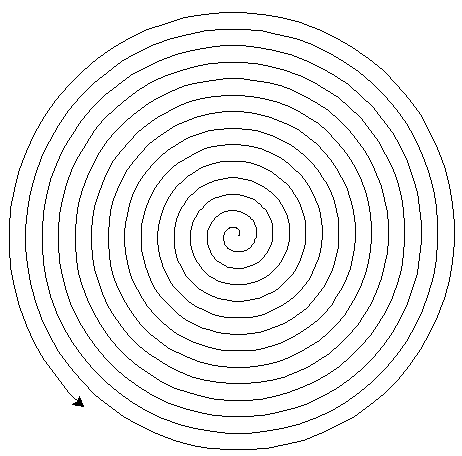
\includegraphics[width=2.0in]{img/spiral}
    \end{figure}

  \item[navigate2.py] Modify \texttt{navigate.py} from last week so that,
    rather than performing each action as it is entered, it stores the inputs in a
    list and runs them all at once after the ``stop'' command has been given.

  \item[sorted.py] Take in numbers as input until ``stop'' is entered. As you
    take in each number, insert it into a list so that the list is sorted in
    ascending order. That is, look through the list until you find the place
    where the new element belongs, then use \pythoninline{.insert()} to place it
    there. If the number is already in the list, do not add it again. After
    ``stop'' is entered, print out the list. Do not use any of Python's built-in
    sorting functions.

    You cannot use \pythoninline!.sort()! for this exercise.

    Sample:

\begin{verbatimcode}
Input a number: 12
Input a number: 5.2
Input a number: 73
Input a number: 100
Input a number: -5
Input a number: 2.3
Input a number: stop
[-5.0, 2.3, 5.2, 12.0, 73.0, 100.0]
\end{verbatimcode}

\end{description}

\pagebreak
\section{Submitting}

Files to submit:
\begin{itemize}
  \item parity.py (see Section~\ref{subsec:listsex})
  \item splitit.py (see Section~\ref{subsec:stringsex})
  \item ends.py (see Section~\ref{subsec:stringsex})
  \item mix.py (see Section~\ref{subsec:stringsex})
  \item spiral.py (see Section~\ref{subsec:forex})
  \item navigate2.py (see Section~\ref{subsec:forex})
  \item sorted.py (see Section~\ref{subsec:forex})
\end{itemize}

You should submit your code as a tarball. It should contain all files
used in the exercises for this lab. The submitted file should be named
\begin{center}
  \texttt{cse107\_firstname\_lastname\_lab4.tar.gz}
\end{center}

\begin{center}
  \textbf{Upload your tarball to Canvas.}
\end{center}

\end{document}
